\subsection{Naturalize}
This section summarizes the previous work of Allamanis et al.~\cite{naturalize} on the tool Naturalize.
The goal of their work was to automatically infer coding conventions out of some given source code
and then give suggestions to the programmer to better adhere to the found conventions.
They limited their scope to the naming of identifiers and code formatting. 
As this paper focuses on the naming part, the code formatting is excluded in this summary. 
The central concept of Naturalize is to use the well-known N-gram model to learn naming conventions from a given source set. Later this model can be used to suggest better alternative names for identifiers, which are more in line with the trained model. 
\begin{figure}
    \centering
    \graphicspath{{resources/}}  
    \def\svgwidth{0.5\textwidth}
    %% Creator: Inkscape 1.0.2 (e86c870879, 2021-01-15), www.inkscape.org
%% PDF/EPS/PS + LaTeX output extension by Johan Engelen, 2010
%% Accompanies image file 'naturalize_workflow.pdf' (pdf, eps, ps)
%%
%% To include the image in your LaTeX document, write
%%   \input{<filename>.pdf_tex}
%%  instead of
%%   \includegraphics{<filename>.pdf}
%% To scale the image, write
%%   \def\svgwidth{<desired width>}
%%   \input{<filename>.pdf_tex}
%%  instead of
%%   \includegraphics[width=<desired width>]{<filename>.pdf}
%%
%% Images with a different path to the parent latex file can
%% be accessed with the `import' package (which may need to be
%% installed) using
%%   \usepackage{import}
%% in the preamble, and then including the image with
%%   \import{<path to file>}{<filename>.pdf_tex}
%% Alternatively, one can specify
%%   \graphicspath{{<path to file>/}}
%% 
%% For more information, please see info/svg-inkscape on CTAN:
%%   http://tug.ctan.org/tex-archive/info/svg-inkscape
%%
\begingroup%
  \makeatletter%
  \providecommand\color[2][]{%
    \errmessage{(Inkscape) Color is used for the text in Inkscape, but the package 'color.sty' is not loaded}%
    \renewcommand\color[2][]{}%
  }%
  \providecommand\transparent[1]{%
    \errmessage{(Inkscape) Transparency is used (non-zero) for the text in Inkscape, but the package 'transparent.sty' is not loaded}%
    \renewcommand\transparent[1]{}%
  }%
  \providecommand\rotatebox[2]{#2}%
  \newcommand*\fsize{\dimexpr\f@size pt\relax}%
  \newcommand*\lineheight[1]{\fontsize{\fsize}{#1\fsize}\selectfont}%
  \ifx\svgwidth\undefined%
    \setlength{\unitlength}{406.04370117bp}%
    \ifx\svgscale\undefined%
      \relax%
    \else%
      \setlength{\unitlength}{\unitlength * \real{\svgscale}}%
    \fi%
  \else%
    \setlength{\unitlength}{\svgwidth}%
  \fi%
  \global\let\svgwidth\undefined%
  \global\let\svgscale\undefined%
  \makeatother%
  \begin{picture}(1,1.04562071)%
    \lineheight{1}%
    \setlength\tabcolsep{0pt}%
    \put(0,0){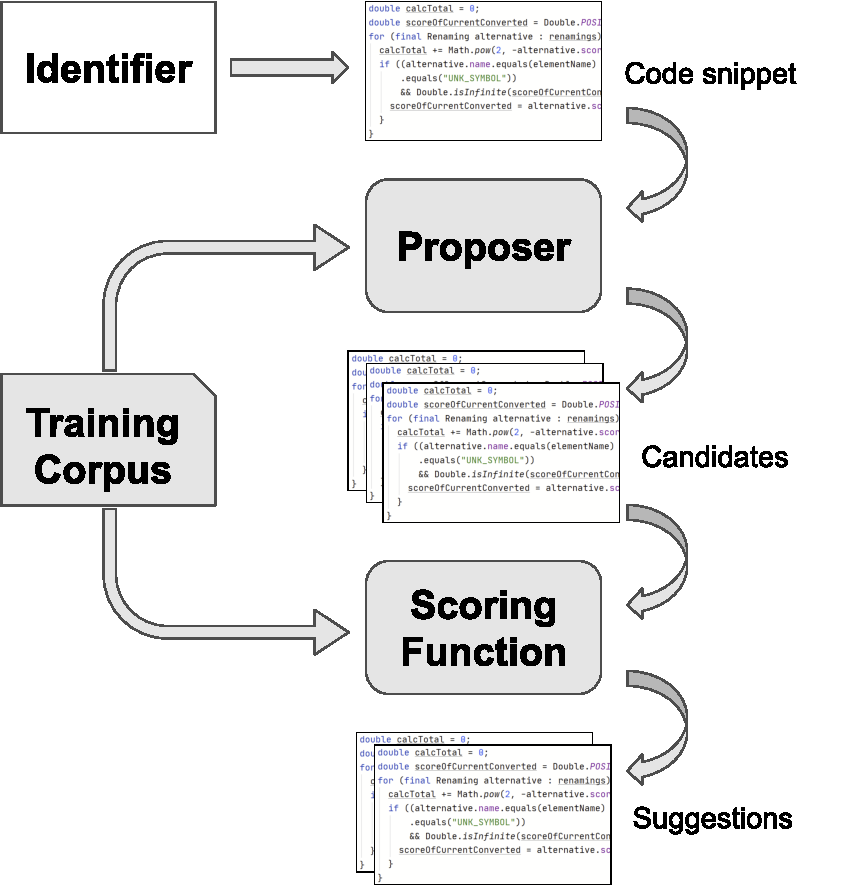
\includegraphics[width=\unitlength,page=1]{naturalize_workflow.pdf}}%
  \end{picture}%
\endgroup%

    \caption{Workflow of Naturalize}
    \label{fig:back_nat_workflow}
\end{figure}

In the learning phase, the tool converts a set of source files into token streams according to the
Java language definition and builds an N-gram model with them. Their findings indicate that a model of
order five is well suited.

After training Naturalize can now suggest alternative names for an identifier. The workflow for this suggestion task is shown in Figure~\ref{fig:back_nat_workflow}.
It starts with a request containing the identifier which should be renamed.
The intuitive idea behind Naturalize is that the name of an identifier depends on the code locations where the identifier is assigned or used. To be able to find those occurrences the initial request contains the AST node of the identifier in the Abstract Syntax Tree
of the current file. This allows Naturalize to find a parent node higher up in the tree, which encompasses all (local) occurrences of the identifier. For example, if the identifier is a local variable, the parent node is the AstNode representing the method, where the variable is defined. Then a code snippet is created, which simply contains the complete textual content of the parent node. This would, in the example above, be the signature and body of the defining method. It is important to mention that Naturalize, at least at the time this paper is being written,
does not include occurrences of identifiers outside of the current class. Now the N-gram model can be used to assign a probability to this code snippet indicating how in line this snippet, and therefore the identifier, is with the rest of the project.

The next step is that the Proposer has to find alternative names for the identifier. For this, the N-gram model is used. The code snippet is scanned and each n-gram, meaning each sub-snippet containing N words, that contains an occurrence of the identifier is extracted. Then the model is checked if it contains N-grams, which are similar to the extracted ones. Similar here means, that the N-gram only differs at the place, where the occurrence of the identifier is present. At this place the similar N-gram contains another identifier. These other identifiers are then used as the candidates for the suggestion. Corresponding code snippets for each candidate can be generated from the original one, by simply replacing the original name with the candidate name. As a last step the scoring function ranks and filters the candidates. This is done by assigning a score to each candidate snippet using the N-gram model.
For filtering a threshold $t$ is introduced. This threshold controls which candidate should be kept by looking at their scores. Only those candidates with
a score greater than at least $t$ in comparison to the original name should be kept. The filtering also includes a parameter $k$, where only the top-$k$ suggestions are kept to not overburden the user with too many suggestions. The final list of suggestions is then presented to the user.

Some details which are not important for this paper were left out of this summary. For example how
Naturalize deals with unique rare names.

\subsection{N-gram smoothing}
Smoothing is an important part of language models that depend on N-grams. The basic equation for the estimated probability of a given N-gram $t=w_1^n=w_i\hdots w_n$ is
\begin{equation}
    P(w_n | w_1^{n-1}) =  \frac{C(w_1^n)}{C(w_1^{n-1})}
\end{equation}
where $C(w_1^n)$ is the number of times the sequence $w_1^n$ is present in the training set.
This simple equation, called the \emph{maximum likelihood} estimate, does not work well, as it assigns a zero score to N-grams that do not occur in the training set. These N-grams should obviously have a probability higher than zero. To solve this problem different smoothing methods can be applied~\cite{smoothingStudy}.

\subsubsection{Katz Smoothing}
Katz smoothing is one of the simplest smoothing techniques. The basic idea is to use a lower order n-gram model (meaning a lower value of n) if the full n-gram occurs less than a given threshold $k$ times in the training set. This is repeated until a low enough n-gram model is found~\cite{katz1987estimation}. As an equation it can be written as:
\begin{equation}
    P(w_n | w_1^{n-1}) = 
    \begin{dcases}
    d_{w_1^{n-1}}\cdot \frac{C(w_1^n)}{C(w_1^{n-1})} & C(w_1^n) > k\\
    \alpha_{w_1^{n-1}} \cdot P(w_n | w_2^{n-1}) & \text{else}
    \end{dcases}
\end{equation}
The value $k$ is mostly, as also in Naturalize, chosen to be 1 and $d$ as well as $\alpha$ are pre-computed values per n-gram~\cite{katz1987estimation}.
\subsubsection{Jelinek and Mercer Smoothing}
Jelinek and Mercer smoothing (JM smoothing) also uses lower-order models to compute the final probability. But instead of using the first lower-order model with a high enough count, JM smoothing interpolates over models of all orders~\cite{smoothingStudy}:
\begin{equation}
    P(w_n | w_1^{n-1})=\lambda_{w_1^{n-1}}\frac{C(w_1^n)}{C(w_1^{n-1})} + (1-\lambda_{w_1^{n-1}})P(w_n | w_2^{n-1})
\end{equation}
Again $\lambda_{w_1^{n-1}}$ are pretrained values. As computing a different value for each $\lambda$ would be to expensive, these values are partitioned into buckets according to $C(w_1^{n-1})$. Every $\lambda_{w_1^{n-1}}$ with the same count is then constrained to have the same value.
Comparing these two methods the main difference between Katz and JM smoothing is that Katz smoothing stops at the first order, where the calculated probability is greater than zero, but JM continues to include lower-order models.